\documentclass[%
reprint,
%superscriptaddress,
%groupedaddress,
%unsortedaddress,
%runinaddress,
%frontmatterverbose, 
%preprint,
%preprintnumbers,
nofootinbib,
%nobibnotes,
%bibnotes,
 amsmath,amssymb,
aps,
%pra,
%prb,
%rmp,
%prstab,
%prstper,
floatfix,
superscriptaddress,
showkeys,
%endfloats,
%onecolumn,
longbibliography
]{revtex4-1}

%TESTE
\usepackage{enumitem}

\usepackage{xr}
\usepackage{tabularx}
\usepackage{booktabs}
\usepackage{graphicx}% Include figure files
% Facilita a resolução de caminhos de figuras
\graphicspath{{figures/}{figures/results/}}
\usepackage{dcolumn}% Align table columns on decimal point
\usepackage{bm}% bold math
\usepackage{microtype}
\usepackage{gensymb}
\usepackage{url}
\usepackage[T1]{fontenc}
\usepackage[utf8]{inputenc}
\usepackage[brazil]{babel}
% Permitir inclusão de PDFs com versão mais alta no output (não resolve a inclusão em si)
\pdfminorversion=7
\pdfobjcompresslevel=0
% add hypertext capabilities e evitar duplicação de anchors
\usepackage[breaklinks, hidelinks, colorlinks=true,linkcolor=blue,citecolor=black,hypertexnames=false]{hyperref}
\usepackage{color, colortbl}
\usepackage[table,xcdraw]{xcolor}
%\usepackage[mathlines]{lineno}% Enable numbering of text and display math
%\linenumbers\relax % Commence numbering lines

%\usepackage[showframe,%Uncomment any one of the following lines to test 
%%scale=0.7, marginratio={1:1, 2:3}, ignoreall,% default settings
%%text={7in,10in},centering,
%%margin=1.5in,
%%total={6.5in,8.75in}, top=1.2in, left=0.9in, includefoot,
%%height=10in,a5paper,hmargin={3cm,0.8in},
%]{geometry}

%VER
% (Removido xcolor duplicado)

\makeatletter
\renewcommand\frontmatter@abstractwidth{\dimexpr0.9\textwidth\relax}
\makeatother

\bibliographystyle{apsrev4-1}
\usepackage{algorithm}
\usepackage{algpseudocode}
\usepackage{multirow}

\makeatletter
\newcommand*{\addFileDependency}[1]{% argument=file name and extension
  \typeout{(#1)}
  \@addtofilelist{#1}
  \IfFileExists{#1}{}{\typeout{No file #1.}}
}
\makeatother

\newcommand*{\myexternaldocument}[1]{%
    \externaldocument{#1}%
    \addFileDependency{#1.tex}%
    \addFileDependency{#1.aux}%
}

\newcommand{\sm}{\scalebox{0.5}[1.0]{\( - \)}}


%VER
\makeatletter
\renewcommand\subparagraph{\@startsection{subparagraph}{5}{\parindent}%
    {3.25ex \@plus1ex \@minus .2ex}%
    {-1em}%
    {\normalfont\normalsize\bfseries}}
\makeatother

\begin{document}
%
\preprint{1}



\title{VessShape: Segmentação 2D de vasos sanguíneos com poucos exemplos explorando priores de forma a partir de imagens sintéticas}
%VessShape: Few-shot blood vessel segmentation using shape priors from synthetic data
%VessShape: Adding shape priors to neural networks for few-shot blood vessel segmentation

\author{Wesley N. Galvão}
\email[]{wesleygalvao@estudante.ufscar.br}
\affiliation{Departamento de Computação, Universidade Federal de São Carlos, São Carlos, SP, Brasil}


\author{Cesar H. Comin}
\email[Autor correspondente: ]{comin@ufscar.br}
\affiliation{Departamento de Computação, Universidade Federal de São Carlos, São Carlos, SP, Brasil}

\date{\today}% It is always \today, today,
             %  but any date may be explicitly specified

\begin{abstract}
% maximum of 250 words

A segmentação semântica de vasos sanguíneos é uma tarefa importante em análise de imagens médicas, mas seu progresso é frequentemente limitado pela escassez de grandes conjuntos de dados anotados e pela fraca generalização dos modelos entre diferentes modalidades de imagem. Um ponto-chave é a tendência das Redes Neurais Convolucionais (CNNs) de aprenderem atributos baseados em textura, o que limita o desempenho quando aplicadas a novos domínios com características visuais distintas. Hipotetizamos que aproveitar priores geométricos da forma dos vasos, como sua natureza tubular e ramificada, pode levar a modelos mais robustos e eficientes em termos de dados. Para investigar essa ideia, introduzimos o VessShape, uma metodologia para gerar conjuntos de dados sintéticos 2D em larga escala projetados para induzir um viés de forma em modelos de segmentação. As imagens do VessShape contêm geometrias tubulares geradas proceduralmente, combinadas com ampla variedade de texturas de primeiro plano e de fundo, incentivando os modelos a aprenderem pistas de forma em vez de texturas. Demonstramos que um modelo pré-treinado com VessShape alcança forte desempenho em segmentação com poucos exemplos em dois conjuntos de dados reais de domínios diferentes, necessitando de apenas quatro a dez amostras para fine-tuning. Além disso, o modelo apresenta capacidades notáveis em zero-shot, segmentando vasos em domínios não vistos sem qualquer treino específico no destino. Nossos resultados indicam que o pré-treinamento com um viés de forma pronunciado pode ser uma estratégia eficaz para contornar a escassez de dados e melhorar a generalização na segmentação de vasos sanguíneos.

\end{abstract}

\keywords{Segmentação de vasos sanguíneos, viés de forma, adaptação de domínio, aprendizado com poucos exemplos}

\maketitle
\thispagestyle{plain}
%\ohead*{\pagemark}

\section{Introdução}
\label{sec:introduction}

A segmentação semântica de vasos sanguíneos é uma área ativa de pesquisa, impulsionada pela demanda por análises precisas e automatizadas de imagens médicas em tecidos humanos e animais. Um grande desafio nessa tarefa é o processo trabalhoso de anotação manual, que exige conhecimento especializado para criar máscaras de segmentação acuradas. Esse gargalo de anotação levou à escassez de conjuntos de dados em larga escala, limitando tanto o treinamento de modelos de aprendizado profundo quanto o desenvolvimento de novos métodos. Por exemplo, conjuntos públicos amplamente utilizados como DRIVE \cite{Staal2004} e CHASE\_DB1 \cite{Fraz2012ensemble} contêm apenas algumas dezenas de imagens anotadas cada. Embora esforços recentes tenham introduzido novos conjuntos de dados \cite{jin2022fives, fhima2024lunet}, a disponibilidade de coleções grandes e diversas ainda é limitada. Esse problema é agravado por mudanças substanciais de domínio entre diferentes modalidades de imagem, como fotografias de fundo de olho e microscopia do córtex cerebral. Variações em textura, densidade e calibre dos vasos dificultam a capacidade de modelos treinados em um domínio generalizarem para outro.

O transfer learning é uma estratégia comum para lidar com essas limitações. Ao reaproveitar representações aprendidas em um domínio fonte, modelos podem obter melhor desempenho em um domínio alvo, mesmo com poucos dados. Técnicas como fine-tuning e adaptação de domínio permitem que modelos pré-treinados em grandes conjuntos de imagens naturais, como o ImageNet \cite{JiaDeng2009}, sejam adaptados para tarefas de segmentação biomédica \cite{zoetmulderDomainTaskspecificTransfer2022}.

Entretanto, um risco do transfer learning padrão é o viés intrínseco das CNNs de privilegiar texturas em detrimento de formas geométricas \cite{geirhos2018, islam2021shape}. Esse viés de textura pode limitar a generalização entre domínios com estilos visuais distintos. Estudos mostram que modelos treinados com ênfase em pistas de forma apresentam melhor desempenho e robustez \cite{geirhos2018}. Isso sugere que transferir representações de forma, em vez de atributos ricos em textura, pode ser uma estratégia mais eficaz para segmentação de vasos com poucos exemplos.

A tarefa de segmentação de vasos sanguíneos é particularmente adequada a uma abordagem centrada em forma. A geometria fundamental dos vasos é um prior consistente em diversas modalidades de imagem, de fotografias do fundo de olho a imagens de microscopia do córtex. Embora texturas e outras características visuais variem amplamente entre domínios, a forma subjacente permanece um identificador universal. Por exemplo, um observador humano que aprendeu a identificar vasos em uma modalidade consegue reconhecê-los em outra, como ilustrado na Figura~\ref{f:motivation}.

\begin{figure}[tbp]
    \centering
    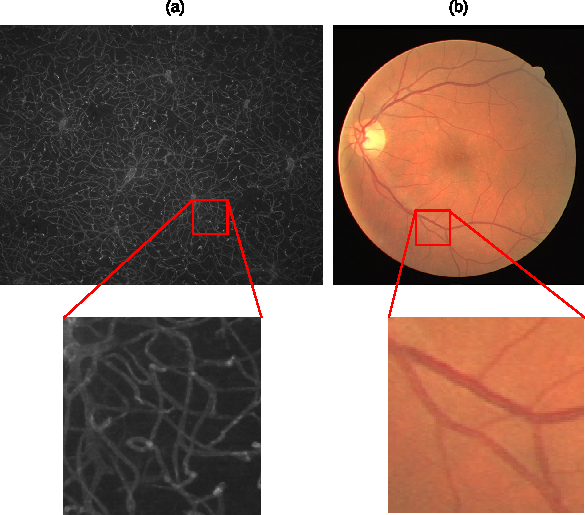
\includegraphics[width=\columnwidth]{figures/vessel_retinal_cortex.pdf}
    \caption{Ilustração da universalidade da forma vascular. (a) Amostra de microscopia por fluorescência do córtex de camundongo. (b) Fotografia de fundo de olho humano. Apesar de apresentarem texturas distintas, os vasos possuem formas semelhantes.}
    \label{f:motivation}
\end{figure}

Com base nessa observação, hipotetizamos que um modelo pré-treinado em um domínio com forte viés de forma necessitará de poucas amostras anotadas para se adaptar a um novo domínio alvo. Esperamos que tal modelo supere um modelo treinado do zero no domínio alvo ao reutilizar de maneira eficaz seus priores geométricos. Para testar essa hipótese, introduzimos o VessShape, uma metodologia para criar conjuntos sintéticos projetados para pré-treinar modelos de segmentação com sensibilidade à forma. O VessShape consiste em imagens 2D com estruturas tubulares semelhantes a vasos, combinadas a uma ampla variedade de texturas de primeiro plano e de fundo. Ao fixar os priores geométricos enquanto diversificamos as texturas, o conjunto incentiva explicitamente os modelos a aprenderem atributos de forma robustos em detrimento de pistas superficiais de textura.

Demonstramos que um modelo pré-treinado com VessShape consegue segmentar com precisão a vasculatura em dois domínios alvo usando apenas quatro a dez amostras anotadas para fine-tuning. Além disso, observamos capacidades notáveis em zero-shot, nas quais o modelo pré-treinado segmenta vasos em novos domínios sem qualquer treino específico.

\section{Trabalhos Relacionados}
\label{sec:related}

Diversos estudos anteriores consideraram priores de forma para segmentação de imagens médicas~\cite{bohlender2021survey,heimann2009statistical,cootes1995active}. Isso é viável quando organelas, células ou órgãos têm formas conhecidas e o processo de segmentação pode assumir uma forma ótima ou critérios adicionais de otimização, como a exigência de bordas suaves. A segmentação por instância é provavelmente a tarefa mais comum na qual priores de forma têm sido explorados. Um desafio particular na identificação de vasos é que geralmente se requer segmentação semântica da imagem. 

Antes da popularização de métodos de aprendizado profundo, priores de forma locais eram a abordagem dominante para segmentação de vasos. Vasos tendem a ter estrutura tubular. Assim, a abordagem usual era desenvolver filtros voltados à identificação de objetos tubulares. Uma linha popular se baseava nos autovalores da matriz Hessiana~\cite{fraz2012blood,sato1998three}. Provavelmente, o método baseado em Hessiana mais conhecido é o filtro de Frangi~\cite{frangi1998multiscale}, que combina autovalores para definir uma medida de tubalidade para os pixels dos vasos. Outra abordagem popular se baseou na definição de templates de linhas ou filtros de Gabor para identificar estruturas vasculares relevantes. Uma limitação importante desses métodos é que a suposição de tubalidade não é válida em pontos de bifurcação e terminação.

Com o surgimento do aprendizado profundo, alguns trabalhos exploraram a inclusão de priores de forma durante o treinamento da rede~\cite{bohlender2021survey}. Priores foram adicionados na entrada da rede usando filtros de vesselness~\cite{affane2022robust,hu2024domain,garret2024deep}, na arquitetura por meio de filtros de vesselness ou Gabor aprendíveis~\cite{chen2023learnable,fu2018frangi,volkov2025modification}, e na saída usando funções de perda conscientes de topologia~\cite{shit2021cldice,hu2019topology,berger2024topologically}. Para redes neurais, uma alternativa mais simples e possivelmente mais flexível é uma abordagem baseada em dados que se concentra em gerar um grande e diverso conjunto de imagens contendo informação a priori sobre a estrutura dos vasos. Nossa proposta difere desses métodos ao usar dados sintéticos para, explicitamente, incutir forte viés de forma enquanto variamos sistematicamente as texturas. A abordagem mais próxima é gerar imagens sintéticas o mais semelhantes possível às amostras do conjunto real. Isso tem sido feito com duas estratégias principais: i) criar um modelo de aparência dos vasos e do fundo da imagem~\cite{tetteh2020deepvesselnet,wittmann2025vesselfm,wittmann2024simulation,mathys2025synthetic} e ii) usar modelos generativos para sintetizar novas amostras a partir de imagens reais.

Abordagens baseadas em modelagem geralmente começam gerando uma topologia biologicamente plausível da vasculatura, seguida da definição de raios variáveis para segmentos vasculares e da inclusão de textura para vasos e fundo. O ruído típico da modalidade de imagem de interesse também é modelado. Um trabalho recente importante nessa direção é um modelo-fundação chamado VesselFM~\cite{wittmann2025vesselfm}, treinado com um grande número de imagens sintéticas e reais.

Quanto a modelos generativos, a maioria dos trabalhos utiliza GANs para criar amostras~\cite{you2022application,andreini2021two,tavakkoli2020novel,costa2017end}. As amostras sintéticas obedecem aos padrões aprendidos a partir do conjunto real, possibilitando a geração de imagens realistas. Trabalhos recentes consideraram modelos de difusão para a mesma tarefa~\cite{go2024generation,guo2025vesseldiffusion,wang2025vastsd}. Alguns estudos também desenvolveram técnicas de transferência de estilo para adaptação de domínio entre diferentes conjuntos~\cite{peng2022unsupervised,chen2023segmentation,chen2021real}.

A principal desvantagem dos trabalhos mencionados é que a rede é treinada para reproduzir forma e textura dos vasos em conjuntos específicos. Mudanças na textura dos vasos, devido a doenças ou a modificações no dispositivo de imagem, podem reduzir o desempenho. Além disso, os modelos precisam ser treinados para modalidades específicas, mesmo quando há pouca anotação disponível. Nossa abordagem visa treinar redes neurais para segmentar qualquer tecido vascular que siga os priores de forma aprendidos com o VessShape.



\section{Metodologia}
\label{s:methodology}

\subsection{O Gerador VessShape}

A geometria das imagens sintéticas no VessShape\footnote{{Repositório de código}: \url{https://github.com/galvaowesley/vess-shape-dataset}} é definida usando curvas de Bézier, que permitem representação flexível e controlada de formas tubulares. Cada segmento vascular é descrito por uma curva de Bézier de ordem $n$ com pontos de controle $\{\mathbf{p}_i\}_{i=0}^n$. A tortuosidade do segmento é ajustada por pequenas perturbações nesses pontos de controle, garantindo geometria realista e diversa. A curva de Bézier $\mathbf{c}(t)$ de um segmento é dada pela Equação~\ref{eq:bezier}, com $t$ variando de 0 a 1.

\begin{equation}
\mathbf{c}(t) \,=\, \sum_{i=0}^{n} \binom{n}{i} (1-t)^{n-i} t^{i} \, \mathbf{p}_i,
\label{eq:bezier}
\end{equation}

Para gerar uma curva, o primeiro ($\mathbf{p}_0$) e o último ($\mathbf{p}_n$) pontos de controle são amostrados uniformemente no domínio da imagem. Os demais pontos de controle são gerados definindo-se $n-1$ pontos igualmente espaçados na reta que conecta $\mathbf{p}_0$ e $\mathbf{p}_n$. Cada um desses pontos é deslocado por uma quantidade aleatória ao longo de um vetor normal $\mathbf{n}_l$. Esse vetor normal é unitário e perpendicular à reta entre $\mathbf{p}_0$ e $\mathbf{p}_n$. O módulo do deslocamento é extraído de uma distribuição uniforme em $[-\delta,\delta]$. Valores menores de $\delta$ produzem curvas mais retas.

Para a geração da máscara binária $M$, cada curva é discretizada por amostragem de pontos em resolução suficiente para capturar sua curvatura, os quais são conectados sequencialmente para formar uma polilinha de 1 pixel na grade da imagem. Em seguida, aplica-se uma dilatação morfológica binária com elemento estruturante em disco de raio $r_0$, conferindo espessura tubular constante aos segmentos. 

Para gerar cada máscara, o número de segmentos $K$, a ordem $n$ das curvas de Bézier, a escala de deslocamento $\delta$ e o raio $r_0$ são amostrados aleatoriamente dentro de intervalos, assegurando grande variedade de formas. A Tabela~\ref{tab:vessshape_params} resume os parâmetros usados na geração do VessShape, com intervalos de amostragem e descrições.

\begin{table*}[t]
\caption{Principais parâmetros usados na geração do conjunto VessShape.}
\label{tab:vessshape_params}
\centering
\begin{tabularx}{\textwidth}{l c X}
\hline
    \textbf{Parâmetro} & \textbf{Intervalo} & \textbf{Descrição} \\
\hline
Número de curvas $K$ & $[1,20]$ & Quantidade de segmentos vasculares gerados por amostra \\
Pontos de controle $n{+}1$ & $[2,20]$ & Controla a complexidade da curva de Bézier \\
Escala de deslocamento $\delta$ (px) & $[50,150]$ & Regula a curvatura/tortuosidade dos segmentos \\
Raio inicial $r_{0}$ (px) & $[1,5]$ & Raio basal do vaso antes da operação de suavização \\
Desfoque do matting $\sigma$ & $[1,2]$ & Desvio-padrão do Gaussiano usado para mesclar primeiro plano e fundo \\

\hline
\end{tabularx}
\end{table*}

Para compor a imagem final $I$ a partir da máscara binária $M$, aplicam-se uma textura de primeiro plano $F$ e uma textura de fundo $B$ aos segmentos vasculares e ao fundo, respectivamente. As texturas são selecionadas aleatoriamente do conjunto ImageNet \cite{JiaDeng2009}. Especificamente, para cada máscara $M$, duas imagens são sorteadas aleatoriamente de duas classes distintas do ImageNet. Em seguida, as imagens são recortadas aleatoriamente e redimensionadas para as dimensões alvo ($H \times W$). Uma máscara alfa $A$ é gerada suavizando $M$ com filtro Gaussiano de desvio-padrão $\sigma$ e normalizando os valores para $[0, 1]$. As texturas são então mescladas de acordo com:

\begin{equation}
I \,=\, A\,F + (1-A)\,B,
\label{eq:compose}
\end{equation}
Essa mescla garante que regiões de vasos ($A \approx 1$) preservem a textura de primeiro plano enquanto regiões não vasculares ($A \approx 0$) mantenham a textura de fundo. 

O parâmetro $\sigma$ controla a suavidade das bordas dos vasos. Exemplos de máscaras e imagens geradas estão na Figura~\ref{f:vessshape_sample}.


\begin{figure}[tbp]
    \centering
    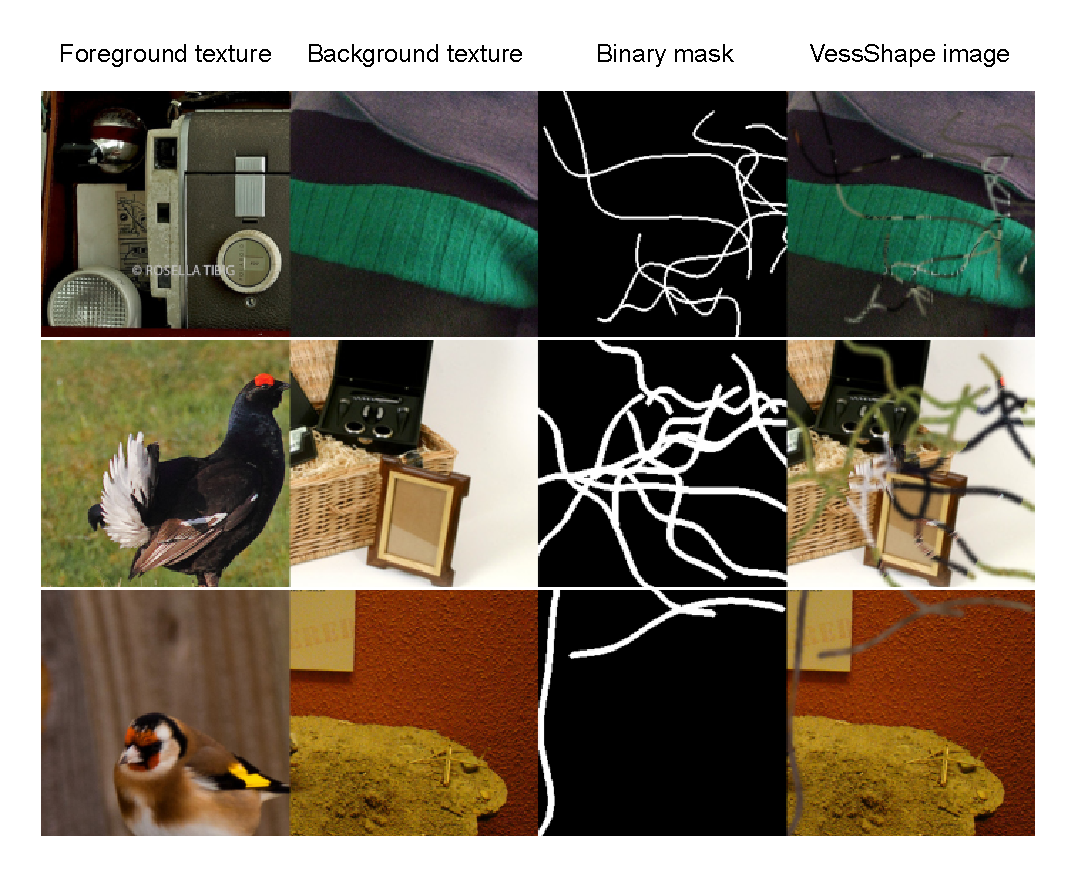
\includegraphics[width=\columnwidth]{figures/results/vessshape_sample.pdf}
    \caption{Exemplos do processo de geração do VessShape. As texturas são amostradas do ImageNet e mescladas conforme máscaras binárias geradas proceduralmente para criar as imagens finais.}
    \label{f:vessshape_sample}
\end{figure}

\subsection{Dados reais para validação}

Para quantificar a utilidade do viés de forma introduzido pelo VessShape, consideramos dois conjuntos de dados de vasos sanguíneos: DRIVE e VessMAP. O DRIVE~\cite{Staal2004} é um padrão amplamente usado para benchmarking de segmentação de vasos retinianos e é composto por 40 fotografias de fundo de olho divididas em 20 para treino e 20 para teste, cada uma com $584\times565$ pixels. Em nossos experimentos, todas as imagens do DRIVE foram convertidas para tons de cinza antes de treino, validação e teste. O VessMAP~\cite{viana2025new} possui 100 imagens, $256\times256$ pixels cada, adquiridas por microscopia de fluorescência do córtex de camundongo. Esse conjunto foi curado para incluir diversas características vasculares desafiadoras, como nível de ruído e contraste inconsistentes, diferentes calibres de vasos, artefatos proeminentes e variações de intensidade dentro das estruturas vasculares.

Os dois conjuntos provêm de modalidades de imagem fundamentalmente distintas, resultando em características diferentes. As imagens de fundo de olho do DRIVE, que capturam toda a retina, possuem organização global clara, incluindo marcos como o disco óptico. As amostras também contêm muitos vasos muito finos, de difícil segmentação. Em contrapartida, as imagens do VessMAP são vistas altamente ampliadas de pequenas regiões corticais e não têm organização global discernível. As bordas dos vasos geralmente são menos definidas do que no DRIVE. Outra diferença é que, sem qualquer processamento, os vasos no VessMAP são claros sobre fundo escuro, enquanto no DRIVE os vasos são escuros sobre fundo claro. A Figura~\ref{f:drive_vessmap_samples} mostra exemplos de cada conjunto.

\begin{figure}[tbp]
    \centering
    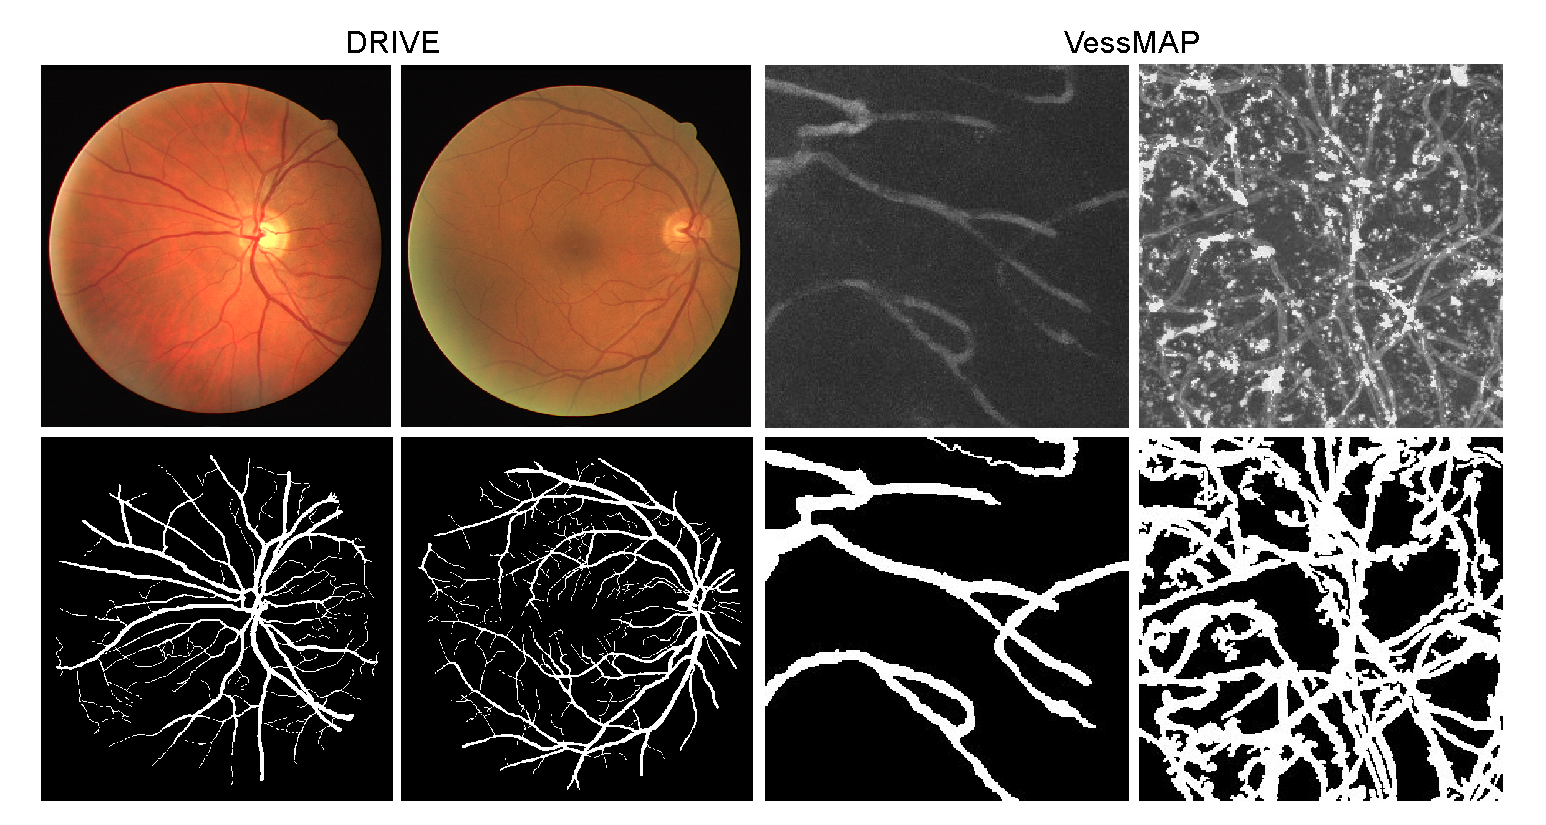
\includegraphics[width=\columnwidth]{figures/results/drive_vessmap_samples.pdf}
    \caption{Amostras dos conjuntos DRIVE e VessMAP e suas respectivas máscaras de referência.}
    \label{f:drive_vessmap_samples}
\end{figure}

\subsection{Arquiteturas de modelo e estratégias de treinamento}

Adotamos a arquitetura U-Net com design encoder-decoder simétrico e conexões de atalho entre estágios correspondentes. Comparamos dois modelos, um com encoder ResNet18 e outro com ResNet50 \cite{he2016deep}. Os modelos foram instanciados a partir do pacote Python \textit{Segmentation Models Pytorch}\footnote{\url{https://github.com/qubvel/segmentation_models.pytorch}}.

Consideramos dois cenários de treinamento. No primeiro, o treinamento é feito do zero separadamente em DRIVE e VessMAP, estabelecendo o baseline. O segundo cenário consiste em pré-treinamento no VessShape seguido de fine-tuning em DRIVE e VessMAP para medir a transferência e a eficiência amostral das representações aprendidas. Esses dois cenários envolvem três procedimentos: i) pré-treinamento no VessShape, ii) fine-tuning nos dados reais, e iii) treinamento do zero nos dados reais. A seguir descrevemos esses procedimentos.

\subsection{Pré-treinamento no VessShape}

O pré-treinamento no VessShape visa expor o modelo a ampla variedade de geometrias tubulares, mantendo a textura como pista secundária. Cada amostra de treino é gerada sob demanda. Esse embaralhamento contínuo de aparência, combinado a regras geométricas estáveis, deve injetar forte viés de forma enquanto desencoraja memorização de texturas. O modelo é otimizado minimizando a perda de entropia cruzada sobre esse conjunto sintético efetivamente infinito. 

Pré-treinamos dois modelos U-Net com encoders ResNet18 e ResNet50, chamados VSUNet18 e VSUNet50. O VSUNet18 foi treinado em aproximadamente 7,1 milhões de imagens sintéticas por 8,6 horas, enquanto o VSUNet50 foi treinado em cerca de 53,0 milhões de imagens por 78,3 horas. Normalização por canal usando estatísticas do ImageNet foi aplicada a todas as entradas. Para avaliação nessa etapa, usamos conjuntos de validação e teste pré-gerados do VessShape com 9.000 e 200 imagens, respectivamente. A Tabela~\ref{tab:vs_hparams} lista os hiperparâmetros. A Tabela~\ref{tab:vessshape_results_percent} resume o desempenho no VessShape. Todas as execuções foram feitas em uma estação com 24 vCPUs e uma GPU NVIDIA GeForce RTX 3090.

\begin{table}[t]
    \caption{Hiperparâmetros de pré-treinamento usados no VessShape.}
    \label{tab:vs_hparams}
    \centering
    \begingroup
    \small
    \setlength{\tabcolsep}{6pt}
    \renewcommand{\arraystretch}{1.15}
    \begin{tabular}{l l l}
        \hline
        \textbf{Hiperparâmetro} & \textbf{VSUNet50} & \textbf{VSUNet18} \\
        \hline
        Tamanho do batch & 96 & 192 \\
        Taxa de aprendizado & $10^{-3}$ & $10^{-2}$ \\
        Weight decay & $10^{-4}$ & 0.0 \\
        \hline
    \end{tabular}
    \endgroup
\end{table}

\begin{table}[t]
    \caption{Desempenho das variantes VSUNet após pré-treinamento no VessShape. Valores, em porcentagem, são média $\pm$ desvio-padrão no conjunto de teste fixo do VessShape.}
    \label{tab:vessshape_results_percent}
    \centering
    \begingroup
    \small
    \setlength{\tabcolsep}{6pt}
    \renewcommand{\arraystretch}{1.15}
    \begin{tabular}{l r r}
        \hline
        \textbf{Métrica} & \textbf{VSUNet50} & \textbf{VSUNet18} \\
        \hline
        Dice & $86.1 \,\pm\, 2.2$ & $85.9 \,\pm\, 7.7$ \\
        Acc & $96.0 \,\pm\, 0.8$ & $95.6 \,\pm\, 3.7$ \\
        IoU & $75.8 \,\pm\, 3.2$ & $76.1 \,\pm\, 9.6$ \\
        Prec & $78.0 \,\pm\, 3.7$ & $77.4 \,\pm\, 9.6$ \\
        Rec & $96.4 \,\pm\, 1.2$ & $97.4 \,\pm\, 1.8$ \\
        \hline
    \end{tabular}
    \endgroup
\end{table}



\subsection{Fine-tuning}

Desenvolvemos um protocolo sistemático de fine-tuning\footnote{Código (pré-treinamento VessShape + fine-tuning com poucos exemplos): \url{https://github.com/galvaowesley/vess-shape-experiments} } para treino com poucos exemplos em conjuntos 2D de vasos, aplicado aqui a DRIVE e VessMAP. O objetivo é quantificar ganhos de desempenho conforme aumenta o número de exemplos rotulados usados na adaptação. Para as variantes VSUNet, sempre partimos dos pesos pré-treinados no VessShape.

Para cada conjunto $D$, dividimos as imagens em três subconjuntos disjuntos: $\mathcal{V}_{\text{train}}$, o pool de imagens rotuladas elegíveis para amostragem few-shot; $\mathcal{V}_{\text{val}}$, usado para ajustes auxiliares; e $\mathcal{V}_{\text{test}}$, retido para avaliação final. Para DRIVE, usamos 16 imagens em $\mathcal{V}_{\text{train}}$, 4 em $\mathcal{V}_{\text{val}}$ e 20 em $\mathcal{V}_{\text{test}}$. Para VessMAP, adotamos 60, 20 e 20, respectivamente.

Para aplicar fine-tuning com amostragem progressiva, definimos um conjunto ordenado de tamanhos $\mathcal{N} = \{ n_1, n_2, \ldots, n_K \}$ com $n_1 = 1$ e $n_K = n_{\mathcal{V}_{\text{train}}}$. Para cada $n \in \mathcal{N}$ realizamos $R$ execuções independentes e, em cada execução $r$, amostramos sem reposição um subconjunto de treino:
\[
\mathcal{V}^{(n,r)}_{\text{train}} = \text{sample}(\mathcal{V}_{\text{train}}, n)
\]

Para cada $n$, mantemos o conjunto de amostras já usadas e priorizamos amostras ainda não utilizadas. Se não houver novas amostras (para $n$ grandes ou $R$ alto), repetições são permitidas. Esse procedimento assegura execuções de treino o mais diversas possíveis.

Cada subconjunto $\mathcal{V}^{(n,r)}_{\text{train}}$ é usado para realizar fine-tuning do modelo $S$ vezes ($s=1,\ldots,S$). Otimizamos a perda de entropia cruzada em $\mathcal{V}^{(n,r)}_{\text{train}}$ e monitoramos o desempenho em $\mathcal{V}_{\text{val}}$ após cada época. O último checkpoint é avaliado em $\mathcal{V}_{\text{test}}$. Essa abordagem permite decompor a variância em: (i) variabilidade de treino condicionada à combinação fixa de imagens (dentro de $(n,r)$) e (ii) variabilidade entre diferentes combinações de imagens (entre $r$).

Neste trabalho, definimos $R=5$ e $S=3$. As sequências de tamanhos $\mathcal{N}$ são $\{1,2,4,6,8,10, 12, 14, 16\}$ para DRIVE e $\{1,2,4,6,8,10, 12, 14, 16,18,20\}$ para VessMAP. Também consideramos o caso zero-shot ($n=0$), em que o modelo pré-treinado é avaliado diretamente em $\mathcal{V}_{\text{test}}$ sem qualquer adaptação a $D$. 


\subsection{Treino do zero nos conjuntos reais}

Estabelecemos um baseline treinando modelos diretamente em DRIVE e VessMAP sem pré-treinamento sintético. Denotamos esses modelos por U-Net18 e U-Net50; o protocolo de treinamento é o mesmo do fine-tuning. A única diferença é a ausência do pré-treinamento no VessShape, expondo a rede a uma fase inicial mais ruidosa e potencialmente mais dependente de textura.

Não definimos caso zero-shot para U-Nets, pois não há estado inicial útil antes de observar ao menos uma imagem rotulada. As curvas few-shot e o regime com todas as amostras permitem quantificar: (i) o ganho absoluto proporcionado pelo viés de forma do VessShape; (ii) a diferença de velocidade de convergência conforme $n$ cresce. Assim, a comparação VSUNet versus U-Net isola o efeito do viés de forma mantendo os demais fatores controlados.


\section{Resultados}
\label{s:results}

Conduzimos análise quantitativa baseada nas curvas de desempenho dos modelos em função do número de exemplos anotados. Os principais resultados estão na Figura~\ref{f:results_charts}. Escolhemos o índice Dice como métrica principal por ser amplamente utilizada em segmentação médica. A Tabela~\ref{tab:combined_fewshot_percent} resume os valores de Dice, além de outras métricas-chave, para zero-shot e few-shot ao longo de execuções repetidas.

\begin{table*}[t]
    \caption{Segmentação com poucos exemplos e em zero-shot no VessMAP e DRIVE. Valores, em porcentagem, são média $\pm$ desvio-padrão sobre execuções repetidas avaliadas no conjunto de teste de cada conjunto. Avaliações zero-shot decorrem de única inferência e, portanto, têm desvio-padrão zero.}
    \label{tab:combined_fewshot_percent}
    \centering
    \begingroup
    \small
    \setlength{\tabcolsep}{4pt}
    \renewcommand{\arraystretch}{1.15}
    \begin{tabular}{l c l l l l l l}
        \hline
        \textbf{Conjunto} & \textbf{\#Exemplos} & \textbf{Modelo} & \textbf{Dice} & \textbf{Acc} & \textbf{IoU} & \textbf{Prec} & \textbf{Rec} \\
        \hline
        \multirow{10}{*}{DRIVE} & \multirow{2}{*}{0} & VSUNet18 & $\mathbf{65.6} \,\pm\, 0.0$ & $90.7 \,\pm\, 0.0$ & $49.0 \,\pm\, 0.0$ & $62.9 \,\pm\, 0.0$ & $69.9 \,\pm\, 0.0$ \\
         &  & VSUNet50 & $36.7 \,\pm\, 0.0$ & $88.8 \,\pm\, 0.0$ & $23.0 \,\pm\, 0.0$ & $72.8 \,\pm\, 0.0$ & $27.5 \,\pm\, 0.0$ \\
         \cline{2-8}
         & \multirow{4}{*}{1} & VSUNet18 & $\mathbf{75.9} \,\pm\, 0.7$ & $94.1 \,\pm\, 0.2$ & $61.2 \,\pm\, 0.9$ & $78.7 \,\pm\, 2.1$ & $74.1 \,\pm\, 1.9$ \\
         &  & VSUNet50 & $75.7 \,\pm\, 1.3$ & $93.9 \,\pm\, 0.6$ & $61.1 \,\pm\, 1.6$ & $77.3 \,\pm\, 4.6$ & $75.4 \,\pm\, 3.9$ \\
         &  & UNet18 & $68.2 \,\pm\, 5.4$ & $91.9 \,\pm\, 1.6$ & $52.3 \,\pm\, 5.8$ & $71.7 \,\pm\, 7.9$ & $69.0 \,\pm\, 11.8$ \\
         &  & UNet50 & $68.1 \,\pm\, 4.6$ & $91.6 \,\pm\, 3.1$ & $52.3 \,\pm\, 5.0$ & $72.2 \,\pm\, 9.9$ & $69.0 \,\pm\, 11.0$ \\
         \cline{2-8}
         & \multirow{4}{*}{16} & VSUNet18 & $79.4 \,\pm\, 0.0$ & $95.0 \,\pm\, 0.0$ & $65.8 \,\pm\, 0.0$ & $83.3 \,\pm\, 0.4$ & $76.2 \,\pm\, 0.3$ \\
         &  & VSUNet50 & $\mathbf{79.9} \,\pm\, 0.1$ & $95.2 \,\pm\, 0.0$ & $66.6 \,\pm\, 0.1$ & $84.6 \,\pm\, 0.3$ & $76.2 \,\pm\, 0.4$ \\
         &  & UNet18 & $78.5 \,\pm\, 0.3$ & $94.6 \,\pm\, 0.1$ & $64.7 \,\pm\, 0.4$ & $79.5 \,\pm\, 0.5$ & $78.1 \,\pm\, 0.4$ \\
         &  & UNet50 & $78.8 \,\pm\, 0.2$ & $94.7 \,\pm\, 0.1$ & $65.0 \,\pm\, 0.2$ & $80.7 \,\pm\, 0.6$ & $77.4 \,\pm\, 0.4$ \\
        \hline
        \multirow{10}{*}{VessMAP} & \multirow{2}{*}{0} & VSUNet18 & $\mathbf{75.7} \,\pm\, 0.0$ & $88.6 \,\pm\, 0.0$ & $61.6 \,\pm\, 0.0$ & $84.6 \,\pm\, 0.0$ & $69.6 \,\pm\, 0.0$ \\
         &  & VSUNet50 & $61.4 \,\pm\, 0.0$ & $81.7 \,\pm\, 0.0$ & $47.2 \,\pm\, 0.0$ & $74.6 \,\pm\, 0.0$ & $60.5 \,\pm\, 0.0$ \\
         \cline{2-8}
         & \multirow{4}{*}{1} & VSUNet18 & $\mathbf{58.9} \,\pm\, 8.0$ & $70.5 \,\pm\, 20.5$ & $45.5 \,\pm\, 8.8$ & $67.5 \,\pm\, 20.5$ & $73.8 \,\pm\, 14.8$ \\
         &  & VSUNet50 & $56.9 \,\pm\, 6.3$ & $70.8 \,\pm\, 20.3$ & $43.9 \,\pm\, 7.1$ & $68.3 \,\pm\, 20.8$ & $70.0 \,\pm\, 16.7$ \\
         &  & UNet18 & $48.8 \,\pm\, 2.7$ & $67.4 \,\pm\, 18.4$ & $36.2 \,\pm\, 3.2$ & $68.2 \,\pm\, 20.4$ & $62.2 \,\pm\, 21.0$ \\
         &  & UNet50 & $46.6 \,\pm\, 2.0$ & $66.5 \,\pm\, 18.1$ & $34.3 \,\pm\, 2.5$ & $67.4 \,\pm\, 20.6$ & $60.4 \,\pm\, 21.5$ \\
         \cline{2-8}
         & \multirow{4}{*}{20} & VSUNet18 & $\mathbf{84.3} \,\pm\, 1.3$ & $90.1 \,\pm\, 2.1$ & $73.9 \,\pm\, 1.8$ & $82.5 \,\pm\, 4.9$ & $88.8 \,\pm\, 4.8$ \\
         &  & VSUNet50 & $83.7 \,\pm\, 2.0$ & $90.5 \,\pm\, 2.5$ & $73.2 \,\pm\, 2.6$ & $85.1 \,\pm\, 3.2$ & $85.0 \,\pm\, 2.7$ \\
         &  & UNet18 & $76.9 \,\pm\, 6.2$ & $88.0 \,\pm\, 3.4$ & $64.5 \,\pm\, 7.5$ & $86.4 \,\pm\, 4.5$ & $73.7 \,\pm\, 9.4$ \\
         &  & UNet50 & $77.6 \,\pm\, 3.7$ & $88.0 \,\pm\, 3.5$ & $65.3 \,\pm\, 4.6$ & $85.5 \,\pm\, 4.1$ & $75.2 \,\pm\, 5.1$ \\
        \hline
    \end{tabular}
    \endgroup
\end{table*}

\begin{table*}[t]
    \caption{Dice (média $\pm$ desvio-padrão) sobre execuções repetidas para segmentação com zero e poucos exemplos nos conjuntos DRIVE e VessMAP. O cenário \textit{zero-shot} aplica-se apenas às variantes VSUNet. Os valores em negrito indicam o melhor desempenho para um determinado número de amostras de treinamento.}
    \label{tab:combined_fewshot_dice_models}
    \centering
    \begingroup
    \small
    \setlength{\tabcolsep}{6pt}
    \renewcommand{\arraystretch}{1.15}
    \begin{tabular}{l r r r r r}
        \hline
        \textbf{Conjunto} & \textbf{\#Amostras} & \textbf{VSUNet18} & \textbf{VSUNet50} & \textbf{UNet18} & \textbf{UNet50} \\
        \hline
        \multirow{3}{*}{DRIVE}
            & 0  & $\mathbf{65.6} \pm 0.0$ & $36.7 \pm 0.0$ & --- & --- \\
            & 1  & $\mathbf{75.9} \pm 0.7$ & $75.7 \pm 1.3$ & $68.2 \pm 5.4$ & $68.1 \pm 4.6$ \\
            & 16 & $79.4 \pm 0.0$ & $\mathbf{79.9} \pm 0.1$ & $78.5 \pm 0.3$ & $78.8 \pm 0.2$ \\
        \hline
        \multirow{3}{*}{VessMAP}
            & 0  & $\mathbf{75.7} \pm 0.0$ & $61.4 \pm 0.0$ & --- & --- \\
            & 1  & $\mathbf{58.9} \pm 8.0$ & $56.9 \pm 6.3$ & $48.8 \pm 2.7$ & $46.6 \pm 2.0$ \\
            & 20 & $\mathbf{84.3} \pm 1.3$ & $83.7 \pm 2.0$ & $76.9 \pm 6.2$ & $77.6 \pm 3.7$ \\
        \hline
    \end{tabular}
    \endgroup 
\end{table*}

As curvas da Figura~\ref{f:results_charts} revelam diferenças no comportamento de treino entre as variantes VSUNet e os modelos treinados do zero (U-Net). Em ambos os conjuntos, os VSUNets começam com vantagem significativa no regime few-shot, alcançando diferença de 7 a 10 pontos percentuais no Dice com apenas uma amostra. Além disso, as curvas dos modelos pré-treinados sobem mais rápido e convergem antes. Em contraste, os U-Nets exibem aprendizado mais lento e prolongado. Essa diferença também se acentua ao analisar a variância entre execuções, tipicamente menor nos VSUNets. No regime com todas as amostras, quando todo o conjunto é utilizado, as métricas ficam mais próximas, mas uma lacuna de desempenho permanece, indicando que o viés de forma adquirido com VessShape continua trazendo benefícios mesmo com mais dados rotulados.

\begin{figure*}[tbp]
    \centering
    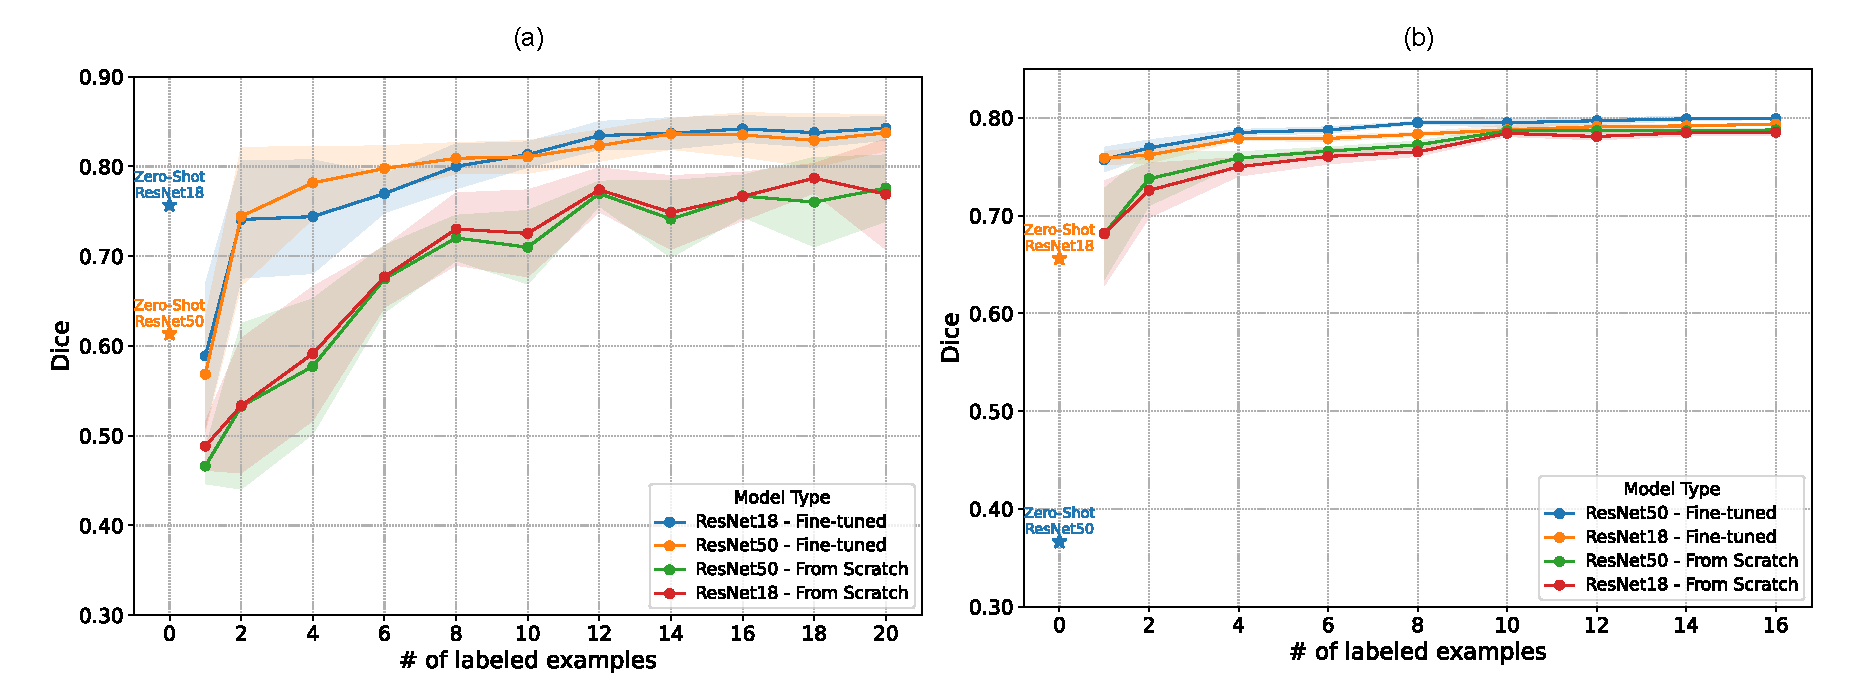
\includegraphics[width=\textwidth]{figures/results/results_charts.pdf}
    \caption{Desempenho em Dice para poucos exemplos e zero-shot em (a) DRIVE e (b) VessMAP. As curvas mostram a média do Dice sobre $R{=}5$ execuções e $S{=}3$ repetições para cada tamanho $n$. As áreas sombreadas representam o desvio-padrão entre execuções. O quadro inserido mostra o Dice zero-shot ($n{=}0$) para VSUNet50 em DRIVE, muito inferior aos demais cenários.}
    \label{f:results_charts}
\end{figure*}

Um fenômeno contraintuitivo ocorre na Figura~\ref{f:results_charts}(b), para VessMAP, em que o desempenho dos VSUNets diminui ao passar de zero-shot para one-shot, antes de se recuperar e superar o zero-shot com mais amostras. Esse comportamento pode decorrer de esquecimento catastrófico \cite{MCCLOSKEY1989109}, quando o fine-tuning com um conjunto muito pequeno leva o modelo a esquecer parte do conhecimento prévio. No entanto, com mais dados, o modelo se recupera e até melhora, sugerindo que o viés de forma inicial é robusto e pode ser reforçado.

A queda em one-shot também foi documentada em modelos de grande escala como o CLIP \cite{Radford2021LearningTV}. O CLIP apresenta forte capacidade zero-shot por ter aprendido regras prévias acessíveis via prompts como "a photo of a {label}". No nosso caso, o pré-treinamento no VessShape induz um prior de forma que funciona de modo análogo a esse conhecimento explícito. Em contrapartida, ao fazer fine-tuning com uma única amostra, o modelo é forçado a otimizar os pesos com informação muito limitada, que inclui não apenas a forma desejada, mas detalhes específicos da instância, como ruído e textura. Isso produz overfitting: em vez de aprender atributos relevantes do novo domínio, o modelo tende a memorizar detalhes específicos desse exemplo único.

Contudo, esse fenômeno não é observado no DRIVE, sugerindo que o prior de forma inicial não está tão alinhado ao domínio do DRIVE. Assim, a primeira amostra traz informação nova e útil, ajudando o modelo a ajustar seus pesos de maneira benéfica, em vez de causar overfitting. De modo semelhante, o modelo se beneficia de mais exemplos, como em \ref{f:results_charts}(a). Uma explicação possível para o menor desempenho é que o desfoque aplicado no VessShape tende a gerar vasos mais espessos do que os do DRIVE. Ajustar parâmetros para refletir melhor os vasos retinianos pode trazer ganhos. Entretanto, as amostras do VessShape usadas foram criadas sem considerar conjuntos específicos, pois o objetivo aqui é avaliar o potencial de priores genéricos de forma para pré-treinamento.

Nossa análise é complementada por avaliação qualitativa das segmentações geradas. A Figura~\ref{f:results_fewshots_drive} ilustra diferenças entre os resultados dos modelos e o impacto do viés de forma. Para o DRIVE, o VSUNet18 zero-shot consegue segmentar corretamente vasos espessos e delinear a estrutura vascular principal, enquanto o VSUNet50 apresenta muitos falsos negativos. Com apenas uma amostra, ambos os VSUNets se adaptam rapidamente, e o VSUNet50 passa a segmentar melhor vasos finos, como destacado pelo retângulo vermelho. As variantes U-Net também segmentam a estrutura principal e a região de interesse com qualidade razoável no exemplo avaliado. Com 16 amostras, as diferenças visuais entre os modelos tornam-se mínimas, convergindo para resultados semelhantes.

\begin{figure*}[tbp]
    \centering
    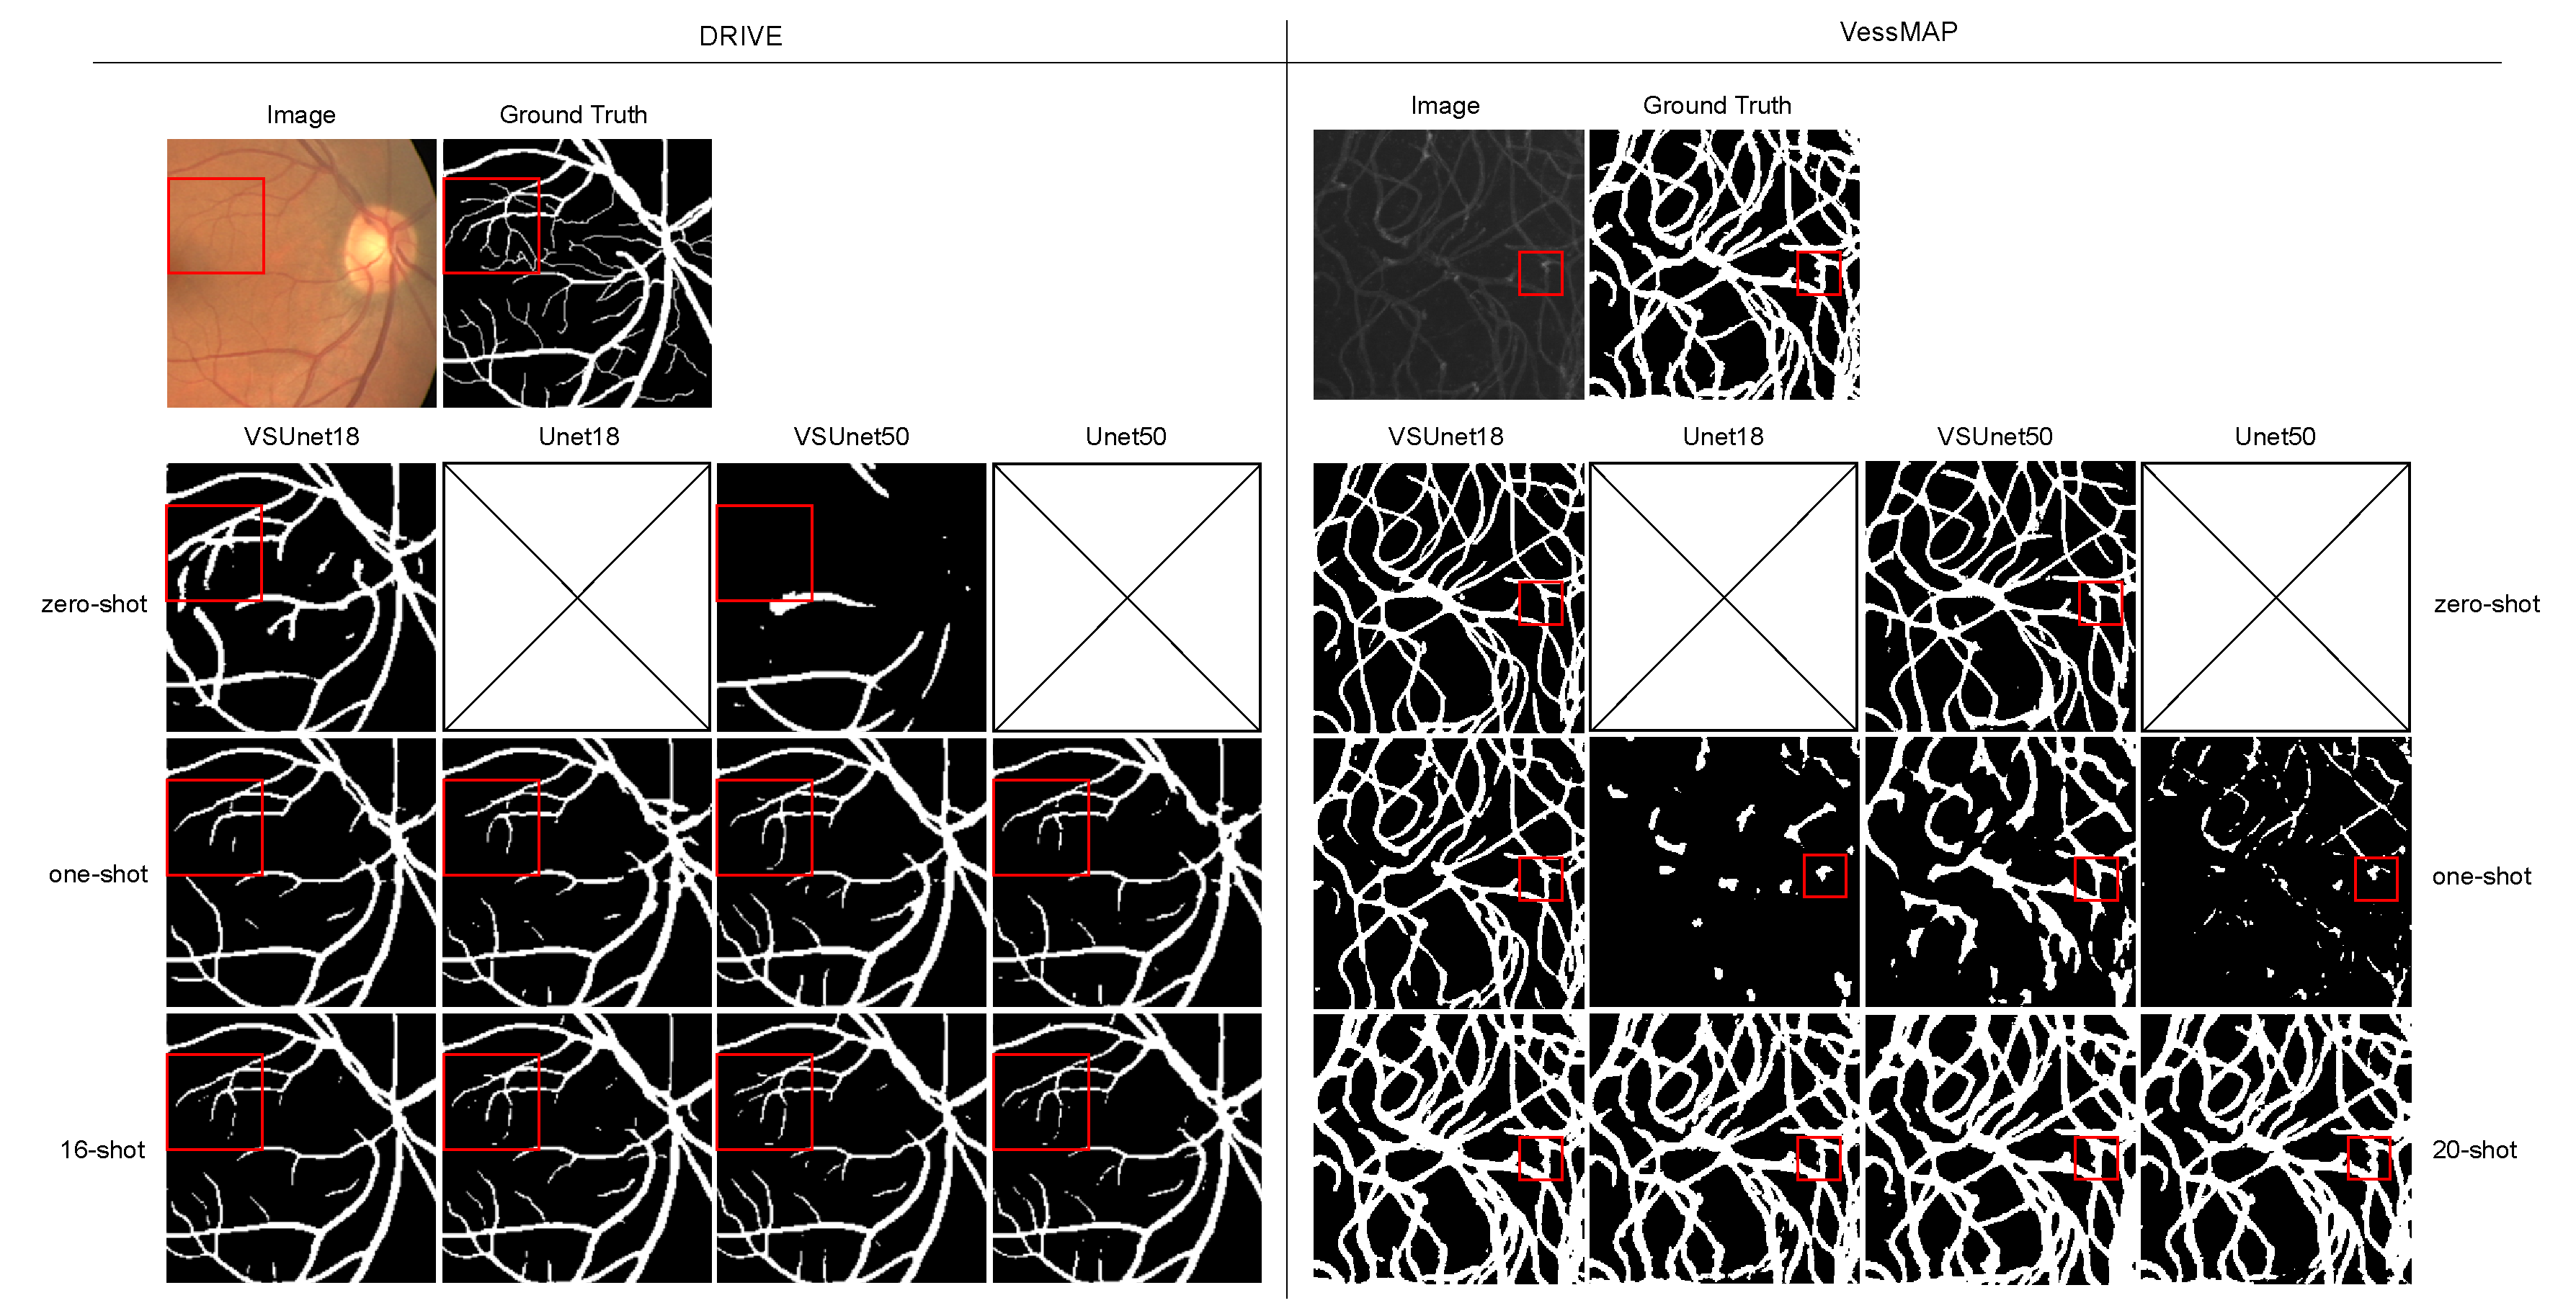
\includegraphics[width=\textwidth]{figures/results/results_fewshots.pdf}
    \caption{Comparação visual qualitativa do desempenho de segmentação em DRIVE e VessMAP. A figura mostra as saídas das variantes VSUNet e U-Net em diferentes regimes: zero-shot, one-shot e few-shot (16 para DRIVE e 20 para VessMAP). Para U-Nets, não há saída zero-shot. Em vermelho destacamos regiões de interesse para facilitar a comparação: uma área com vasos de baixo calibre no DRIVE e uma dilatação vascular no VessMAP.}
    \label{f:results_fewshots_drive}
\end{figure*}

Para o VessMAP, a região em vermelho mostra uma dilatação vascular com mudança brusca de intensidade. Os VSUNets zero-shot capturam a topologia geral, mas não a forma da dilatação. O cenário one-shot confirma a queda de desempenho, com saídas descontínuas nos VSUNets e segmentações de baixa qualidade nos U-Nets, sem conhecimento prévio. Ainda assim, o VSUNet18 já indica um refinamento inicial da geometria da dilatação. Com 20 amostras, todos melhoram de forma significativa, embora os U-Nets ainda exibam pequenas falhas de continuidade em comparação aos mapas mais coesos dos VSUNets.

Apesar de menor e treinado com bem menos dados que o VSUNet50, o VSUNet18 apresentou desempenho zero-shot superior e se manteve competitivo em todos os experimentos, oferecendo um bom equilíbrio entre eficiência e generalização.

Um dos resultados mais relevantes é a capacidade de generalização, evidenciada pelo desempenho zero-shot. Os modelos conseguem segmentar vasos em domínios visualmente distintos sem qualquer treino específico. No VessMAP, os vasos têm alta intensidade sobre fundo escuro; no DRIVE, são escuros sobre fundo claro. O VSUNet18 segmenta um grande número de vasos em ambos os domínios sem fine-tuning. Essa habilidade de generalização sugere que o modelo aprendeu representações de forma robustas, aplicáveis independentemente das características visuais do domínio.



\section{Conclusão}
\label{s:conclusion}

Propusemos uma estratégia focada em incutir forte viés de forma em modelos de aprendizado profundo por meio de pré-treinamento no VessShape, um gerador de dados sintéticos em larga escala. Ao combinar geometrias simples e universais, semelhantes a vasos, com texturas altamente diversas, o VessShape incentiva os modelos a aprenderem priores de forma robustos em detrimento de características específicas de um domínio.

Nossos experimentos demonstraram a eficácia dessa abordagem. Um modelo pré-treinado com VessShape alcançou forte desempenho few-shot em dois conjuntos reais distintos e desafiadores, DRIVE (fotografia de fundo de olho) e VessMAP (microscopia do córtex), necessitando de poucas amostras anotadas para se adaptar a novos domínios. Além disso, o modelo exibiu capacidades notáveis em zero-shot, identificando estruturas vasculares sem qualquer fine-tuning. Esses resultados confirmam nossa hipótese de que explorar um prior geométrico é uma estratégia eficaz para melhorar a eficiência de dados e a robustez a mudanças de domínio.

Embora nosso trabalho atual se concentre em priores genéricos, o VessShape é flexível o suficiente para ser ajustado às características de uma vasculatura específica. Por exemplo, seus parâmetros podem ser calibrados para gerar vasos mais finos e nítidos, típicos de imagens retinianas, em contraste com o VessMAP. Consideramos essa otimização específica por domínio uma direção promissora, pois nosso objetivo primário aqui foi avaliar o impacto de priores gerais de forma.

Há diversas frentes para trabalhos futuros. A geração geométrica atual do VessShape, baseada em curvas de Bézier, pode ser estendida para incluir topologias vasculares mais complexas e biologicamente plausíveis, como bifurcações reais e estruturas em rede. Além disso, estender o Vesshape para 3D permitiria aplicar essa estratégia de pré-treinamento a modalidades volumétricas, como CT e MRI. Estudos futuros também podem explorar a aplicação de pré-treinamento centrado em forma a outras estruturas tubulares na biologia, como neurônios ou vias aéreas.

Nosso trabalho destaca um princípio interessante: para tarefas de segmentação com priores de forma fortes e consistentes, focar em características geométricas centrais pode ser uma estratégia de pré-treinamento mais eficaz e generalizável do que tentar imitar a aparência de um único domínio alvo.


\section*{Declaração de Ética}

Este estudo foi conduzido usando conjuntos de dados públicos, anonimizados, e não envolveu novos experimentos com seres humanos ou animais. Portanto, em conformidade com diretrizes institucionais e nacionais, esta pesquisa foi isenta de apreciação por comitê de ética, e não se aplica exigência de consentimento informado.

\section*{Agradecimentos}
Este estudo foi financiado, em parte, pela Fundação de Amparo à Pesquisa do Estado de São Paulo (FAPESP), Brasil. Processo número \#2025/04800-9.

\bibliography{references}

\end{document}
